\usepackage{xspace}
\newcommand{\ps}{phylesystem\xspace}
\newcommand{\otol}{Open Tree of Life\xspace}
\newcommand{\nexson}{otNexSON\xspace}
\newcommand{\js}{JavaScript\xspace}
\newcommand{\authorswaffil}{Emily Jane McTavish$^{1*}$,
 James Pettengill$^{2}$, Steve Davis$^{2}$, Hugh Rand$^{2}$, Errol Strain$^{2}$, Marc Allard$^{2}$,
 Ruth E. Timme$^{2}$
}
\newcommand{\affil}{$^{1}$ Department of Ecology and Evolutionary Biology, University of Kansas, Lawrence KS, USA\\
$^{2}$ Center for Food Safety and Nutrition, Food and Drug Administration, College Park, MD\\
*Corresponding author
}

\begin{document}
\firstpage{1}
\mytitle{Tree to Reads}{TreeToReads - a pipeline for simulating raw reads from phylogenies}

\myauthor{McTavish \textit{et~al}}{\authorswaffil}
\myaddress{\affil}
\history{Received on XXXXX; revised on XXXXX; accepted on XXXXX}
\editor{Associate Editor: XXXXXXX}
\maketitle
\posttitle{\authorswaffil}{\affil}


\begin{abstract}
\textbf{Summary:}
Using genome-wide single nucleotide polymorphism (SNP)-based methods for tracking pathogens has become standard practice in academia and for public health agencies.
Multiple computational approaches call variants by mapping short read data against a reference genome, filtering those variants for quality, then concatenating them into a sequence matrix for down-stream phylogenetic analysis.
However, despite our knowledge of the parameters that affect whether a SNP is called, we lack methods for determining the effects of read mapping choices on whether the correct tree has been recovered.
To resolve this problem, we offer a program, TreeToReads, which can generate raw read data from mutated genomes simulated under a known phylogeny.
This simulation pipeline allows direct comparisons of simulated and observed data to the same reference genome, and therefore can be used to test the phylogenetic effects of distance to that reference genome.
At each step of these simulations, researchers can vary parameters of interest (e.g., topology, model of sequence evolution, and read coverage) to assess the robustness of a given result.
Such critical assessments of the accuracy and robustness of analytical pipelines are essential to progress in both research and applied settings. 

\textbf{Availability and implementation:}
Source code, examples, and a tutorial are available at \url{https://github.com/snacktavish/TreeToReads}. 

\textbf{Contact:} ejmctavish@gmail.com
\textbf{Supplementary information:}
Input and output files for the case study are available in the online supplementary information.
\end{abstract}

\section*{Introduction}
Whole genome sequencing (WGS) now allows researchers to trace ancestry among samples that differ by only a few mutations.
Phylogenetic trees inferred from WGS data are a valuable tool for tracing the ancestry of closely related lineages in pathogen outbreaks.
However, these estimates of shared ancestry may rely on only a handful of data points.
When the resulting phylogenetic trees are used by public heath agencies to make public health decisions, e.g. to define the scope of foodborne outbreaks \citep{jackson_implementation_2016},
to identify the source of these outbreaks \citep{hoffmann_tracing_2015, dallman_phylogenetic_2016, allard_practical_2016} and where appropriate to follow-up with regulatory or legal actions, it is particularly important to ensure that the WGS analysis methods used are validated.

One potential source of error is biases in which variable sites (single nucleotide polymorphisms, or SNPs)
are detected from analysis of the sequencing read data. SNP ascertainment biases can be caused by various factors.
These biases can be affected by analysis parameters, such as using missing data cutoffs \citep{huang_unforeseen_2014} or read filtering artifacts \citep{li_toward_2014}.
Read mapping issues due to choice of reference genome \citep{bertels_automated_2014} and different mapping algorithms \citep{pightling_choice_2014} can also result in biases in which variable sites are detected.
Phylogenetic error can be exacerbated by interaction among dataset biases and analytic choices;
for example, using a model of evolution developed for sequence data on a panel of exclusively variable sites \citep{lewis_likelihood_2001}, or choosing an inappropriate model of evolution \citep{sullivan_are_1997}.

Despite the sheer quantities of genomic data, it is possible that these types of biases could affect phylogenetic conclusions.
If these errors are systematic, analyses can converge to support an incorrect result with high bootstrap confidence.
In order to adopt data analysis pipelines for the regulatory environment it is necessary to understand potential biases in sequence analysis pipelines and validate their use.
Simulations are a useful approach to investigating potential biases. 
Without validated \emph{in silico} modeling, food safety scientists have to rely on benchmark datasets where the truth can never be truly known.

To help solve this problem, we present TreeToReads (TTR), a software tool for simulating realistic patterns of sequence variation across phylogenies.
These data may be used to assess the robustness of evolutionary inferences from whole genome data against potential biases inherent in data collection and analysis pipelines.
Two key aspects of TreeToReads differentiate it from existing simulation alternatives.
First, the variable sites follow a user-specified phylogeny, resulting in more realistic evolutionary patterns.
Second, those variable sites are placed in the context of an observed or `anchor' genome, which is represented as the tip on that phylogeny.
Together, this combination allows researchers to make direct comparisons of WGS read mapping between their observed and simulated reads, 
and thus makes TTR appropriate for testing the effects of distance to a reference genome on phylogenetic inference from genomic data.
That 'anchor genome' can be used as a reference genome for read mapping, or mapping can be tested against other empirically-observed genomes.
In the case of empirically-observed genomes, what separates the reference data from the simulated data constitutes real evolutionary history.
Making direct read mapping comparisons to assess reference genome effects cannot be done using alternative simulation software.



\begin{figure*}[trees]
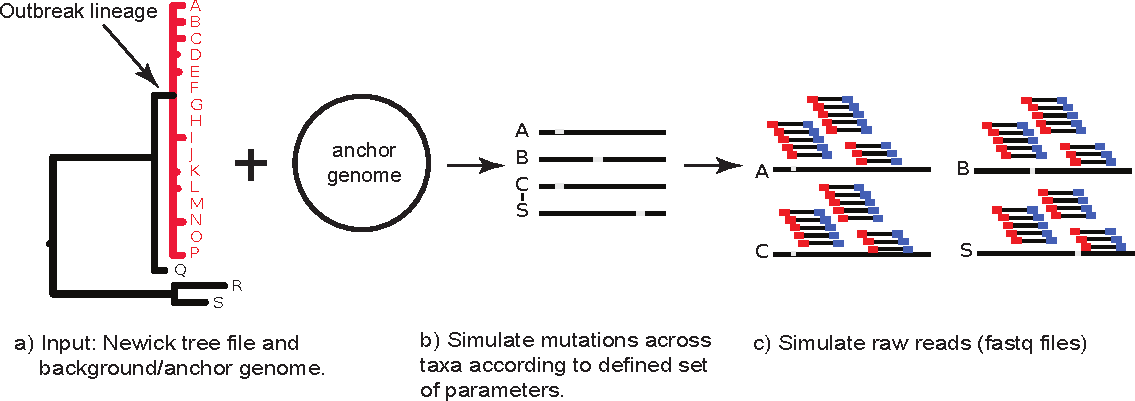
\includegraphics[width=6.5in]{TTR-figure}
\caption{Schematic of the TreeToReads procedure}
\label{scheme}
\end{figure*}

\section*{Methods}
The TreeToReads pipeline generates short read data from genomes simulated along an input phylogeny (Figure 1).
The software is written in Python and requires a configuration file and two input files - a phylogeny with branch lengths and a FASTA formatted genome sequence that serves as the `anchor genome'.
The user specifies parameter settings (e.g., number of variable sites to simulate and nucleotide substitution model parameters) in a configuration file.
The branch lengths of the user provided phylogeny determine the relative number of mutations on each branch and the probability that a single site is affected by multiple mutational events.
To account for the ascertainment bias inherent in estimating phylogenies from panels of variable sites, the total number of variable sites is determined by a user input parameter, not the branch lengths.
The pipeline uses Seq-Gen \citep{rambaut_seq-gen:_1997} to simulate variable sites along the input phylogeny.
Phylogeny formats are standardized using DendroPy \cite{sukumaran_dendropy:_2010}.
These sites are then distributed across the anchor genome. 
The locations of mutations are either drawn from a uniform distribution, or clustered according to parameters of an exponential distribution specified in the configuration file.
This procedure creates an output folder for each tip in the tree that contains the simulated genomes (FASTA files).
A user-specified tip will consist of the input anchor genome without any mutations.
Using these simulated genomes, TreeToReads calls the read simulation software, ART, \citep{huang_art:_2012} to generate Illumina MiSeq paired-end reads.
The user can apply a default sequence error model, or use the configuration file to specify an error model generated for observed data.
TreeToReads currently supports automated generation of Illumina paired end reads.
For other read types, the simulated genome files may be used outside of TreeToReads with any ART parameter configuration.
Alternatively, if RAD-seq like data are desired other raw-read generators such as SimRAD \citep{lepais_simrad:_2014} can be used on the simulated genomes from TTR.
If ART is invoked in TreeToReads the program will output a folder labeled 'fastq'
containing directories labeled with the names of each tip from the simulation tree, in which the simulated reads are deposited in .fastq.gz and .sam formats.
A file with the location and nucleotide state of each mutation within each tip is also provided. 


\section{Case Study}
To demonstrate TreeToReads, we tested the effects of sequence coverage on SNP calling and recovery of a phylogeny.
As a case study we used whole genome read data from ten Salmonella enterica Bareilly sequences,
associated with a 2010 outbreak, and the observed phylogeny inferred from those data \citep{hoffmann_tracing_2015}.
We were interested in determining whether we would be able to capture the phylogenetic split that distinguishes those isolates belonging to the outbreak from isolates which were not part of that outbreak.
We used a completed Salmonella enterica genome (CFSAN000189, GenBank: CP006053.1) as the anchor sequence, and simulated 150 variable sites under the GTR model.
Based on the locations of variable sites in the observed sequence data, the distances between locations for 20\%  of the variable sites were drawn from an exponential distribution with a 125bp mean.
The locations for the rest of the variable sites were drawn from a uniform distribution across the genome. The read error profile was based on the observed outbreak sequence data
We simulated data using four different sequence coverage settings, with an average of 1, 5, 15, and 30 reads at each site.
We analyzed the resulting four short read datasets using the SNP pipeline from the Food and Drug Administration, Center for Food Safety And Nutrition (FDA CFSAN) to identify SNPS in each simulated dataset \citep{davis_cfsan_2015}. 
The CFSAN SNP Pipeline uses reference-based alignments to create a matrix of SNPs for a given set of samples.
We inferred the phylogeny for each data set using RAxML, under the ASC GTRCAT model, which corrects for including only variable sites \citep{stamatakis_raxml_2014}.
At coverage levels of 5, 15, and 30 reads per site the correct phylogeny was consistently inferred.
However, at an average coverage of 1 read per site it was not possible to correctly infer the lineage leading to the outbreak clade.
This simple test case demonstrates how TreeToReads can be applied to analyze the effects of a given parameter, sequence coverage in this case, on phylogenetic inferences from WGS reads. 

\section*{Comparison to existing software}
Although many software tools can simulate sequence data, no existing tools combine phylogenetic relationships with observed genomic sequences.
TreeToReads is designed to test the effects of multiple parameters on phylogenetic inference.
In addition, TreeToReads provides a pipeline to simulate next-gen sequencing reads from a phylogenetic tree using an observed error model.
Using an anchor genome as a tip in the simulated tree means that simulated and empirical data can be mapped to the same reference genome, providing direct comparisons of inferences.
In addition, the reference genome does not need to be the anchor genome on which the simulations are based.
If a different reference is used, the biological evolution separating the anchor genome from the reference genome includes real evolutionary processes affecting read mapping to genomes in a testable framework.
Alternatively, the user can use the simulated data to test reference-free methods for phylogenetic inference, such as wgMLST , kSNP \citep{gardner_when_2013}.

Seq-Gen \citep{rambaut_seq-gen:_1997}, used to generate the variable sites in the TreeToReads pipeline, uses a full generalized time reversible (GTR) model of evolution  with parameters specified by the user.
However, on its own, Seq-Gen generates random sequences based on the model of evolution and therefore does not incorporate observed genomic context.
Consequently, reads from Seq-Gen-simulated genomes cannot be mapped to observed reference genomes.
This is also true for other simulators of more complex evolutionary processes, such as Indelible \citep{fletcher_indelible:_2009} and SWGE \citep{arenas_simulation_2014}.
Although these simulators include complex evolutionary processes not simulated in TreeToReads, such as indels and recombination across lineages, those processes are not drivers of variation in closely related outbreak lineages.
Other sequence simulation software, such as ALF \citep{dalquen_alfsimulation_2012} and Indel Seq-gen \citep{strope_indel-seq-gen:_2007}, simulate evolution forward in time, starting from an input  genome representing the root of the phylogeny.
However, in empirical data the reference genome is not an ancestor - it is always a present day relative.
Anchoring an observed genome to a tip in a tree using TreeToReads allows us to test choices about selection of reference genomes in a way that is directly comparable to empirical data. 



\section*{Conclusions}
Existing genomic simulation software packagescannot provide a phylogenetic perspective in simulation testing of assembly and alignment tools.
TreeToReads allows researchers to test the joint effects of multiple parameter values on the ability of any analysis pipeline to recover the signal and infer the correct tree.
Simulating data that spans these parameters can validate methods for reconstructing phylogenies directly from short-read data, which is especially useful for public health agencies tracking emerging pathogens. 

%%Don't forget to thank Torsten and Lee Katz
\section*{Declartions}
\bibliography{note}
\end{document}
